\section{Introduction}
\label{sec:intro}

% %!TEX root = ../../main.tex
\begin{figure}[t]
    \centering 
    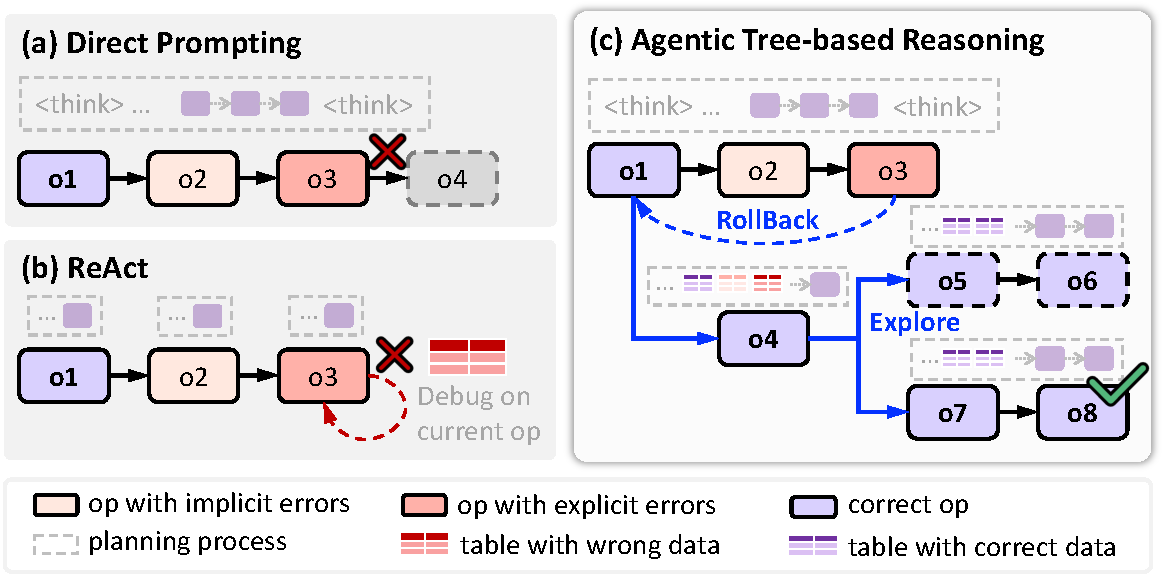
\includegraphics[width=0.99\columnwidth]{figures/fig/prompting_methods.pdf}
    % \vspace{-1em}
    \caption{Comparison of Different Inference Engine.
    }
    \label{fig:prompting_methods}
    % \vspace{-1em}
\end{figure}
%!TEX root = ../../main.tex
\begin{figure}[t]
    \centering 
    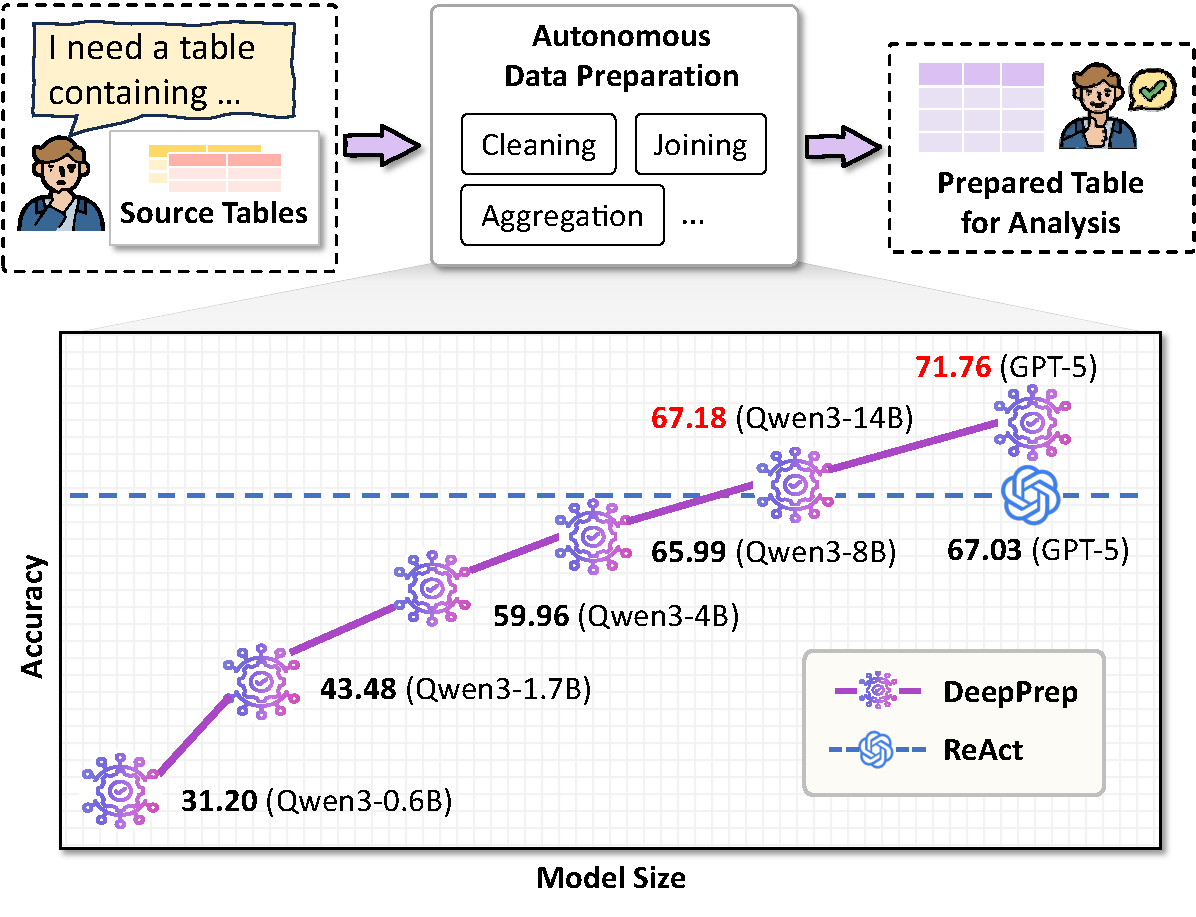
\includegraphics[width=0.85\columnwidth]{figures/fig/introduction_experiment.pdf}
    \vspace{-1em}
    \caption{Overview of Autonomous Data Preparation (Top) and Performance of \sys (Bottom).}
    \label{fig:introduction_experiment}
    \vspace{-1em}
\end{figure}
%!TEX root = ../../main.tex
\begin{figure*}[!t]
    \centering 
    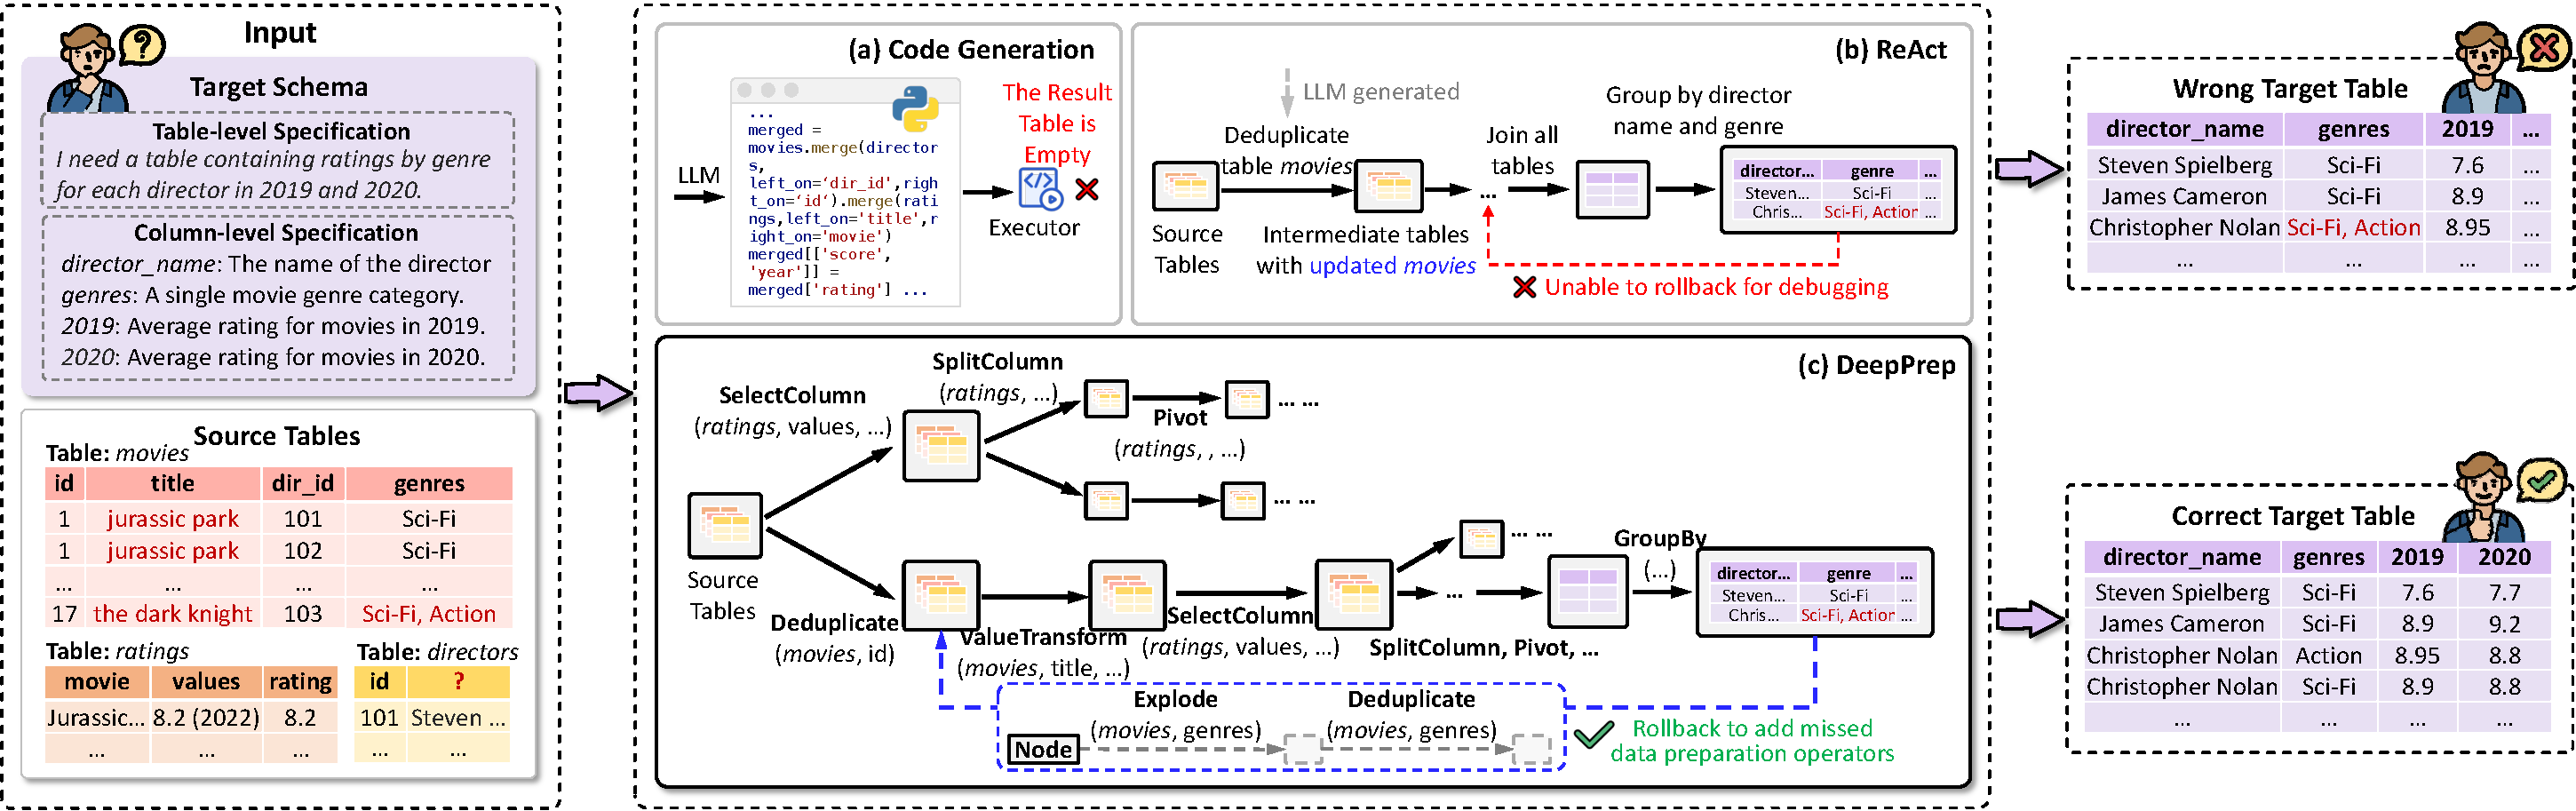
\includegraphics[width=0.95\textwidth]{figures/fig/introduction_example.pdf}
    \vspace{-1em}
    \caption{An illustrative example highlighting the core idea of \sys.
(a) Code generation makes decisions without grounding in intermediate execution results.
(b) ReAct-style approaches follow linear reasoning with limited ability to revise earlier decisions.
(c) \sys applies a tree-based structured exploration, which enables backtracking to resolve non-local errors.
    }
    \label{fig:introduction_example}
    \vspace{-1em}
\end{figure*}

Tabular Data Preparation (DP), the process of transforming raw tables into analysis-ready formats, remains a critical bottleneck in data science, often consuming 60-80\% of the total analysis time~\cite{dasu2003exploratory}. 
In real-world scenarios, the ideal interaction paradigm is \textbf{Natural Language (NL) \nlwhat DP}. As illustrated in Figure~\ref{fig:introduction_experiment},
to process heterogeneous raw tables, the user only needs to provide  high-level analysis requirements (\eg \textit{``I want to analyze director performance...''}). The system should then automatically generate the necessary sequence of DP operations, ranging from data cleaning, table reconstruction, and column transformation. Finally, it yields a prepared table ready for downstream analysis. 

However, existing methods fail to realize this vision. Traditional tools~\cite{barowy2015flashrelate, singh2016blinkfill, he2018transform, gulwani2012spreadsheet, jin2017foofah, heer2015predictive} primarily rely on rigid specifications, e.g. instance data of the target table. They do not understand the high-level ambiguous intent of the user. 

Large Language Models (LLMs) bring opportunities to NL-\nlwhat DP due to remarkable capabilities in NL understanding and code generation. 
% Current LLM-based approaches generally fall into two categories.
The current state-of-the-art (SOTA) approach is CodeGen~\cite{sapkota2025vibe}, in which an LLM-based agent interactively produces and runs code.
While this approach is adaptable, it encounters substantial difficulties in complex DP tasks. As shown in Figure~\ref{fig:introduction_example}(a), CodeGen frequently produces a single code block that encompasses multiple DP operations, without examining the intermediate outcomes. Consequently, when an error occurs (for example, an empty result table), it becomes challenging to determine whether the data was lost during the merge or during text extraction.
Moreover, from an implementation standpoint, the resulting code is often brittle when faced with noisy or imperfect data. Even when the LLM correctly determines the required transformation (for example, capitalizing the first letter of the \texttt{movies.title} column), it usually produces naive code that lacks defensive checks and therefore fails when encountering null values.

% \stitle{Operator-Assisted Data Preparation.}
Inspired by traditional operator-centric approaches (\eg Auto-Tables~\cite{DBLP:journals/pvldb/LiHYWC23}), recent work restricts LLMs to invoking a fixed set of predefined operators. This design offers two advantages that address the issues found in CodeGen.  
First, these encapsulated operators act as the fundamental units of interaction with the environment. The model can immediately examine the outcome after each DP operator is executed, making the DP procedure more controllable and easier to validate.  
Second, by relying on {pre-defined, robust implementations}, the approach sidesteps the brittleness of code generation. This cleanly separates high-level reasoning from low-level execution details, enabling the model to concentrate on {operation planning} instead of dealing with syntax errors or implementation edge cases.

A straightforward realization of such an operator-assisted approach follows the ReAct paradigm~\cite{aksitov2023rest}. This method proceeds in a linear manner, generating each subsequent operator conditioned on the output of the preceding one. Yet, in DP tasks, operators exhibit strong interdependencies, and a suboptimal decision made in an early stage may only surface as a failure several steps later.

\begin{example}
\label{exam:react_issue}
Consider the example shown in Figure~\ref{fig:introduction_example}. Given three tables (``{movies}'', ``{ratings}'', and ``{directors}''), the task is to construct a table that supports analyzing director performance across movie genres using audience ratings. 
% It requires to perform data cleaning, table reconstruction, and column transformation operations on three source tables: ``{movies}'', ``{ratings}'', and ``{directors}''.
As depicted in Figure~\ref{fig:introduction_example}(b), ReAct iteratively generates the \textbf{next} operator to execute the required DP operations. After joining these tables, it then attempts to aggregate the combined data to produce the desired analysis table. However, the resulting table includes multi-category entries such as ``Sci-Fi/Action'' in the ``genre'' column, which violates the user’s specification. This issue arises from insufficient data cleaning performed on the ``movies'' table.
% To fix this errors, it requires to rollback a few steps and perform \texttt{Explode} operation to break up the multi-category cells. While this rollback capabilities can not be provided by such .
\end{example}

This example highlights a typical cin complex DP tasks. Addressing it requires rolling back several steps and performing an \texttt{Explode} operation to split the multi-category cells in the ``movies'' table. However, this functionality cannot be supported by the ReAct method because its reasoning process is linear and append-only.

% \stitle{Agentic Tree-based Reasoning}
To bridge the gap, we propose \bfsys, an agentic tree-based reasoning framework,
% . Instead of greedily selecting the next single step, \sys orchestrating 
which orchestrates the correct operator sequence through a tree structure. Specifically, we define the state of the agent as the collection of historical planning and environment interaction. This state is formulated in a tree structure, denoted as ``state tree''. Based on it, the agent iteratively uses three actions (<analyze>, <expand>, <execute>) to automatically update the state and conduct DP operations.
In each step, \sys first employs {<analyze} to evaluate the state tree and provides a clear plan for the next step. Based on this plan, \sys uses {<expand} to extend a new branch of operators from a specific node. An external executor then executes the new branch and returns interaction results via {<execute}, which are updated into the state tree. Through this automated process, \sys generates an operator tree capable of producing the correct target table. It finally extracts this correct operator pipeline via {<solution} for the final output.

\jie{I used the Writefull AI assistant native to Overleaf (won't use the text body for training their model) to paraphrase all paragraphs before this point. However, I ran out of quota. You may try with yours, purchase it for a month, or use other AI to rephrase. The writing still feels weird. }Through this design, \sys demonstrates two features which can address the \textit{interdependency issue} in ReAct. 
First, the tree-based reasoning paradigm naturally decomposes the complex task into sub-tasks.
% Thus, the operator pipeline required for the each sub-task is much shorter than the origin task. 
This ensures that the reasoning for each sub-task relies only on the relevant local context rather than a noisy global history, preventing errors in one sub-task from affecting others.
Second, the state tree enables {precise backtracking}. 
Unlike ReAct, which relies on a linear, append-only history, \sys explicitly maintains the environment snapshot at each node. This allows the agent to revert to any previous node and start a new path from a clean state, effectively discarding the failed attempt.

% Instead of only debugging on the current operator, \sys can revert to the any previous node where the error originated and explore a new branch to fix it. 

\begin{example}
\label{exam:agentic_tree_based_reasoning}
    Figure~\ref{fig:introduction_example}(c) demonstrates the workflow of \sys. 
    % \textbf{(1) Divide-and-Conquer.} 
    Initially, starting from the root node, the model uses {<analyze} to decompose the complex requirement into sub-tasks. It adopts a divide-and-conquer strategy, sequentially utilizing {<expand} and {<execute} to create three separate branches (sub-trees). Each branch independently performs data cleaning operations on one of the source tables (``{movies}'', ``{ratings}'', and ``{directors}'').
    Subsequently, to integrate the data, \sys extends the operator path by joining the cleaned results from these three branches. Instead of regenerating operators from scratch, \sys effectively extract valid operators from the sub-trees to form a merged table.
    % \textbf{(2) Precise Backtracking.}
    After generating a path that joins all tables and groups by genre, \sys detects an issue in the execution result: the output contains unseparated categories like ``Sci-Fi/Action''. 
    Unlike ReAct which fail to fix this error, \sys analyzes the lineage and pinpoints that the root cause lies in the earlier ``{movies}'' cleaning phase. 
    Consequently, \sys {backtracks} to the specific node in the ``{movies}'' branch before the join operation. It then {expands a new branch} by inserting an {Explode} operator to correctly handle multi-category cells. Finally, \sys re-generates the subsequent join and group operators along this new correct path, successfully producing the target table.
\end{example}

% The above example further illustrates how \sys exhibits these two features. 
Moreover, to scale this reasoning paradigm to complex, real-world DP tasks involving long operator pipelines, we further equip \sys with two critical techniques: \textit{Scalable Data Synthesis} and \textit{Multi-Stage Policy Learning}.

% 这里重点说通过数据集构造让我们的模型支持**多种**操作，**长序列**规划的能力，对比其他方法operator数量少，序列短
% (1) \textbf{Scalable Data Synthesis.} 
Existing datasets focus on single DP task or only involve short sequence of DP operators, which are insufficient for training robust agents. For example, Auto-Table~\cite{DBLP:journals/pvldb/LiHYWC23} only focuses on table reconstruction and only consider cases involving one or two operators. In contrast, practical data preparation involves operators from {multiple DP tasks} including data cleaning, table reconstruction and column transformation~\cite{heer2015predictive} and often requires combining over {a dozen operators} to achieve a practical DP requirement~\cite{2011-wrangler}.
To bridge this gap, we propose a data synthesis method to synthesize DP data involving long-chain DP operations of multiple tasks. 
% , which allows for the scalable synthesis of DP data involving long-chain DP operations from multiple tasks and enables the model to learn complex DP logic. 
Specifically, the synthesized dataset involving operations of column transformation, table reconstruction and data cleaning, with operator pipeline length from 1$\sim$28.

% \fmh{where the validity and quality of each trajectory are strictly guaranteed through execution-based verification.} \jie{analysis operators?quality ?}
% Specifically, we begin with collecting real data analysis requirement from public NL2SQL datasets~\cite{spider_dataset, bird_dataset}, providing several clean and well-formatted input tables and a target table generated by executing the sql query. Then, starting from the input tables, we 

% (2) \textbf{Multi-Stage Policy Learning.} 
The complexity of the task requires \sys to be equipped with long-chain reasoning capabilities, which can not be obtained by simply fine-tuning LLMs~\cite{xie2025logic}. Moreover, although Reinforcement Learning (RL) is demonstrated to be effective to enhance long sequence reasoning capabilities, it suffers from the {sparse rewards} issue where the model fails to roll out correct trajectories during training, making it unable to learn effectively~\cite{gao2024designing}.
To overcome these challenges, we introduce a multi-stage training framework.
First, we design a {progressive cold-start curriculum} to endow the model with the ability to instruction following and initial reasoning capabilities.
Motivated by previous research that dense reward can help improve the training performance~\cite{gao2024designing}, we employ {multiturn RL with a hybrid reward}. By integrating fine-grained evaluation with semantic feedback, our method provides dense signals for effective RL training.

% \stitle{Two Deployment Settings.} 
Furthermore, to meet real-world needs, \sys supports two flexible deployment settings.
First, \textbf{\sysp}, is designed for {plug-and-play} scenarios where users rely on proprietary LLMs (\eg GPT-5) without training resources. As shown in Figure~\ref{fig:introduction_experiment}, by applying our agentic tree-based reasoning via prompting, \sysp significantly enhances the baseline capabilities (surpassing MCTS with GPT-5). 
Second, \textbf{\syst}, caters to scenarios requiring {open-source or private} deployment. By applying our data synthesis and multi-stage training pipeline to further enhance open-source models capabilities on DP tasks, \syst exhibits strong {scaling laws}. As shown in Figure~\ref{fig:introduction_experiment}, the performance of \syst improves consistently with model size, allowing an 8B model to achieve competitive or even better performance comparable to baselines with GPT-5.

In summary, our contributions are as follows:
% \jie{new problem definition?}

    % (1) \textbf{Agentic Tree-based Reasoning Framework.}
    (1) We formally define a new problem of NL-\nlwhat DP (Section~\ref{sec:preliminary}) and introduce an agentic tree-based reasoning framework \sys (Section~\ref{sec:overview}) with two deployment settings (\sysp and \syst) for flexible use.
    
    % propose \sys, a framework leveraging a state tree to maintain the full history of planning and execution, serving as a unified foundation for both prompting (\sysp) and training (\syst) paradigms.
    
    % (2) \textbf{Scalable Synthesis and Training Strategy.} 
    (2) \jie{reverse order? We introduce a scalable data synthesis method (Section~\ref{sec:data_synthesis}) and a multi-stage policy learning method (Section~\ref{sec:agentic_training_framework}) to equip \sys with the capability to handle complex, long-chain DP tasks.}
    
    % (3) \textbf{SOTA Performance and Scalability.} 
    (3) Extensive experiments demonstrate that \sys achieves state-of-the-art performance. \sysp outperforms GPT-5 based baselines (\eg CodeGen), while \syst exhibits robust scaling laws with various model sizes.
    % , validating the effectiveness of our approach across open-source models from 0.5B to 8B parameters.

    (4) \jie{open source issue} We open-source our synthesized datasets, the code for our framework, and a suite of 8 trained data preparation agents (from 0.5B to 8B, catering for scenarios with different computing resources).
    % We also provide an interactive demo to facilitate community testing and deployment.